\begin{itemize}
    \item Location of a point on a line

    \vbdefinition{
        Imagine a world where you can only move in two directions: forward and backward. You can't move left or right, up or down—only along a single straight path. This path is called the x-axis. The x-axis is a horizontal line that extends infinitely in both directions. \\[2mm]
        In this one-dimensional world, we can describe the location of any point using a single number, which we call the coordinate of that point. This number tells us exactly how far along the x-axis the point is from a specific reference point known as the origin. The origin is the center point of the x-axis and has a coordinate of $0$.\\[2mm]
        If a point has a positive coordinate, it means the point is to the right of the origin. If a point has a negative coordinate, it means the point is to the left of the origin. The greater the number, the further the point is from the origin.
    }


        \begin{center}
            \begin{tikzpicture}
                \tzaxes(-5, 0)(5, 0.15){$x$}{}
                \tzticks{-4/$-4$, -3/$-3$, -2/$-2$, -1/$-1$, 0/$0$, 1/$1$, 2/$2$, 3/$3$, 4/$4$}{}
                \tzticks*{-4, -3, -2, -1, 1, 2, 3, 4}{}
            \end{tikzpicture}
            \begin{tikzpicture}
                \tzaxes(-5, 0)(5, 0.15){$x$}{}
                \tzticks{-2.5/$x_1$, 2.5/$x_2$}{}
                \tzticks*{-2.5, 0, 2.5}{}
                \tzline[|<->|]<0, -0.75>(-2.5, 0)(2.5, 0){$x_2 - x_1$}[mb]
            \end{tikzpicture}
        \end{center}

    \item Location of a point in a plane
    \vbdefinition{
        Now, imagine a world where you can move not just forward and backward, but also left and right. This world is two-dimensional, meaning it has two directions or axes along which you can move: the x-axis and the y-axis.\\[2mm]
        The x-axis is a horizontal line that runs from left to right, and the y-axis is a vertical line that runs from bottom to top. These two lines intersect at a point called the origin, which has the coordinates (0, 0).
        In this two-dimensional world, we can describe the location of any point using a pair of numbers called coordinates. These coordinates are written as (x, y):\\[2mm]
        The first number, x, tells us how far along the x-axis the point is from the origin. A positive x value means the point is to the right of the origin, while a negative x value means the point is to the left.
        The second number, y, tells us how far along the y-axis the point is from the origin. A positive y value means the point is above the origin, while a negative y value means the point is below.
    }

        \begin{center}
            \begin{tikzpicture}
                \tzaxes[<->](-5, -2.5)(5, 3.5){$x$}{$y$}
                \tzticks*{-4, -3, -2, -1, 1, 2, 3, 4}{-2, -1, 1, 2, 3}
                \tzticks{-4/$-4$, -3/$-3$, -2/$-2$, -1/$-1$, 1/$1$, 2/$2$, 3/$3$, 4/$4$}{-2/$-2$, -1/$-1$, 1/$1$, 2/$2$, 3/$3$}
                \tzcoor*(0, 0)(O){$O$}[bl]
                \tzcoor*(2, 3)(P){$P(2,3)$}[ar]
                \tzline[|<->|]<0, -0.5>(0, 0)(2, 0){$2$}[mb]
                \tzline[|<->|]<2.5, 0>(0, 0)(0, 3){$3$}[mr]
            \end{tikzpicture}
        \end{center}
% \pagebreak
        % \textbf{Coordinates of a point $P(x, y)$:} \\
        
        \begin{itemize}
            \item \textbf{Distance between two points:}
                \begin{center}
                    \begin{tikzpicture}
                        \tzaxes(-2, -1.5)(7, 4){$x$}{$y$}
                        \tzcoor*(0, 0)(O){$O$}[bl]
                        \tzcoor*(2, 3)(P){$P(x_1, y_1)$}[ar]
                        \tzcoor*(5, 1)(Q){$Q(x_2, y_2)$}[ar]
                        \tzline[dashed](2, 1)(5, 1){$x_2-x_1$}[mb]
                        \tzline[dashed](2, 1)(2, 3){$y_1-y_2$}[ml]
                        \tzline(P)(Q){$d$}[ma]
                        \tzline[|<->|]<0, -0.5>(0, 0)(2, 0){$x_1$}[mb]
                        \tzline[|<->|]<0, -1>(0, 0)(5, 0){$x_2$}[mb]
                        \tzline[|<->|]<-0.5, 0>(0, 0)(0, 1){$y_2$}[ml]
                        \tzline[|<->|]<-1, 0>(0, 0)(0, 3){$y_1$}[ml]
                    \end{tikzpicture}
                \end{center}
                \begin{align*}
                    \intertext{Distance between two points $P(x_1, y_1)$ and $Q(x_2, y_2)$:}
                    \intertext{Using Pythagoras theorem:}
                    \Aboxed{d &= \sqrt{(x_2 - x_1)^2 + (y_2 - y_1)^2}}
                \end{align*}

            \item \textbf{Midpoint of a line segment:}
                \begin{center}
                    \begin{tikzpicture}
                        \tzcoor*(2, 3)(P){$P(x_1, y_1)$}[ar]
                        \tzcoor*(5, 1)(Q){$Q(x_2, y_2)$}[ar]
                        \tzcoor*(3.5, 2)(M){$M(x_m, y_m)$}[ar]
                        \tzline[dashed](2, 1)(5, 1){$x_2-x_1$}[mb]
                        \tzline[dashed](2, 1)(2, 3){$y_1-y_2$}[ml]
                        \tzline(P)(Q)
                        \tzline[dashed](2, 2)(M){$x_m-x_1$}[mb]
                        \tzline[dashed, |<->|]<-1.5, 0>(2, 2)(2, 3){$y_1-y_m$}[ml]
                    \end{tikzpicture}
                \end{center}
                \begin{align*}
                    \intertext{Midpoint of a line segment $P(x_1, y_1)$ and $Q(x_2, y_2)$:}
                    \intertext{From the above diagram, we can see that both the triangles are similar.}
                    \intertext{Therefore,}
                    \frac{y_1-y_m}{y_1-y_2} &= \frac{x_m-x_1}{x_2-x_1} = \frac{PM}{PQ} \\
                    \intertext{As the midpoint divides the line segment into two equal parts,}
                    \frac{y_1-y_m}{y_1-y_2} &= \frac{x_m-x_1}{x_2-x_1} = \frac{1}{2}
                \end{align*}
                \begin{align*}
                    \intertext{Solve for $x_m$ and $y_m$:}
                    \frac{x_m - x_1}{x_2 - x_1} &= \frac{1}{2}  &\text{and}&& \frac{y_1 - y_m}{y_1 - y_2} &= \frac{1}{2} \\
                    x_m - x_1 &= \frac{x_2 - x_1}{2}  &\text{and}&& y_1 - y_m &= \frac{y_1 - y_2}{2} \\
                    x_m &= \frac{x_1 + x_2}{2}  &\text{and}&&  y_m &= \frac{y_1 + y_2}{2}
                \end{align*}
                \begin{align*}
                    \Aboxed{M(x_m, y_m) &= \left(\frac{x_1 + x_2}{2}, \frac{y_1 + y_2}{2}\right)}
                \end{align*}
        \end{itemize}

    \pagebreak

    \item Location of a point in space
    \vbdefinition{
        In a three-dimensional world, we have three axes along which we can move: the x-axis, the y-axis, and the z-axis. The x-axis is a horizontal line that runs from left to right, the y-axis is a vertical line that runs from bottom to top, and the z-axis is a line that runs from front to back. These three axes intersect at a point called the origin, which has the coordinates (0, 0, 0).\\[2mm]
        In this three-dimensional world, we can describe the location of any point using a set of three numbers called coordinates. These coordinates are written as (x, y, z):\\[2mm]
        The first number, x, tells us how far along the x-axis the point is from the origin. A positive x value means the point is to the right of the origin, while a negative x value means the point is to the left.\\[2mm]
        The second number, y, tells us how far along the y-axis the point is from the origin. A positive y value means the point is above the origin, while a negative y value means the point is below.\\[2mm]
        The third number, z, tells us how far along the z-axis the point is from the origin. A positive z value means the point is in front of the origin, while a negative z value means the point is behind.
    }

        \begin{center}
            %\tdplotsetmaincoords{30}{0}
            \begin{tikzpicture}%[tdplot_main_coords]

                % Draw the axes
                \draw[thick,->] (-2,0,0) -- (5,0,0) node[anchor=west]{$x$};
                \draw[thick,->] (0,-2,0) -- (0,4,0) node[above]{$y$};
                \draw[thick,->] (0,0,-2) -- (0,0,5) node[below]{$z$};
            
                % Define the point coordinates
                \coordinate (P) at (3,2,4);
            
                % Draw the point
                \filldraw (P) circle (2pt) node[anchor=south west] {$(x,y,z)$};
            
                % Draw projection lines to the axes
                \draw[dashed] (P) -- (3,2,0);
                \draw[dashed] (P) -- (3,0,4) node[midway, right] {$y$};
                \draw[dashed] (P) -- (0,2,4);
                \draw[dashed] (3,2,0) -- (3,0,0);
                \draw[dashed] (3,2,0) -- (0,2,0);
                \draw[dashed] (3,0,4) -- (0,0,4) node[midway, below] {$x$}; 
                \draw[dashed] (3, 0, 4) -- (3, 0, 0) node[midway, right] {$z$};
                \draw[dashed] (0,2,4) -- (0,2,0);
                \draw[dashed] (0,2,4) -- (0,0,4);
            \end{tikzpicture}
        \end{center}
        \begin{itemize}
            \item \textbf{Distance from origin:}
                \begin{center}
                    \tdplotsetmaincoords{70}{110} % Set the view angles for 3D plot
                    \begin{tikzpicture}[tdplot_main_coords]
                    % Define coordinates for the points
                        \def\xPone{3}
                        \def\yPone{2}
                        \def\zPone{4}

                        % Draw the axes
                        \draw[thick,->] (0,0,0) -- (6,0,0) node[anchor=north east]{$x$};
                        \draw[thick,->] (0,0,0) -- (0,6,0) node[anchor=north west]{$y$};
                        \draw[thick,->] (0,0,0) -- (0,0,4) node[anchor=south]{$z$};

                        % Define the point coordinates
                        \coordinate (P1) at (\xPone,\yPone,\zPone);
                        % Draw the points
                        \filldraw[red] (P1) circle (2pt) node[anchor=south west] {$(x,y,z)$};

                        % Draw projection lines for P1 to the axes
                        \draw[dashed] (P1) -- (\xPone,\yPone,0) node[midway, right] {$z$};
                        \draw[dashed] (0, 0, 0) -- (\xPone, \yPone, 0) node [midway, left] {$\sqrt{x^2+y^2}$};
                        \draw[dashed] (\xPone,\yPone,0) -- (\xPone,0,0) node [midway, below] {$y$};
                        \draw[dashed] (\xPone,\yPone,0) -- (0,\yPone,0) node [midway, right] {$x$};
                        \draw[dashed,red] (0,0,0) -- (P1) node[midway, left] {$d$};
                    \end{tikzpicture}
                \end{center}
                \begin{align*}
                    \intertext{For calculation of $d$, we can use Pythagoras theorem:}
                    \intertext{Imagine $d$ as a hypotenuse of a right-angled triangle with base in x-y plane and height in z-axis, then imagine the base as a hypotenuse of a right-angled triangle with base in x-axis and height in y-axis.}
                    d^2 &= \textit{(base x-y plane)}^2 + \textit{(height z-axis)}^2 \\
                    \intertext{$\textit{(base x-y plane)}^2 = x^2 + y^2$ }
                    d^2 &= x^2 + y^2 + z^2 \\
                    \Aboxed{d &= \sqrt{x^2 + y^2 + z^2}}
                \end{align*}
            
            \item \textbf{Distance between any two points in space:}
                \begin{center}
                    \begin{tikzpicture}
                        \tzcoor*(2, 3, 4)(P){$P(x_1, y_1, z_1)$}[ar]
                        \tzcoor*(7, 1, 2)(Q){$Q(x_2, y_2, z_2)$}[ar]
                        \tzline(P)(Q){$d$}[ma]
                    \end{tikzpicture}
                \end{center}
                \begin{align*}
                    \intertext{Consider two points $P(x_1, y_1, z_1)$ and $Q(x_2, y_2, z_2)$:}
                    \intertext{We can also prove this in similar way using Pythagoras theorem: \hfill (Try yourself)}
                    d &= \sqrt{(x_2 - x_1)^2 + (y_2 - y_1)^2 + (z_2 - z_1)^2} \\
                \end{align*}
            \item \textbf{Midpoint of a line segment:}
                \begin{center}
                    \begin{tikzpicture}
                        \tzcoor*(2, 3, 4)(P){$P(x_1, y_1, z_1)$}[ar]
                        \tzcoor*(7, 1, 2)(Q){$Q(x_2, y_2, z_2)$}[ar]
                        \tzcoor*(4.5, 2, 3)(M){$M(x_m, y_m, z_m)$}[ar]
                        \tzline(P)(Q)
                    \end{tikzpicture}
                \end{center}
                \begin{align*}
                    \intertext{Midpoint of a line segment $P(x_1, y_1, z_1)$ and $Q(x_2, y_2, z_2)$:}
                    \intertext{Again, we can prove this in similar way as we did for 2D: \hfill (Try yourself)}
                    \Aboxed{M(x_m, y_m, z_m) &= \left(\frac{x_1 + x_2}{2}, \frac{y_1 + y_2}{2}, \frac{z_1 + z_2}{2}\right)}
                \end{align*}
        \end{itemize}
\end{itemize}
